\chapter{Mass and Volume}\label{ch:g6:mass-and-volume}

How much lemonade fits in the bottle, and how heavy is the crate of
bottles? Two different questions --- room and stuff --- that
everyday talk cheerfully tangles into one word, ``big''. Science
untangles them: \omterm{def:g6:mass-and-volume:volume}{volume} for the room a thing takes, \omterm{def:g3:measuring-mass:mass}{mass} for the
stuff it holds. Measuring the second, you are an old hand; today we
learn to \omterm{def:g6:measurement-in-science:measuring}{measure} the first --- even for a pebble with no shape a
ruler could love.

\section{Volume: the room a thing takes}

\begin{definition}[Volume]\label{def:g6:mass-and-volume:volume}
The \emph{volume}\index{volume} of a thing is the amount of room it
takes up. \omterm{def:g3:solids-liquids-gases:solid}{Solids}, \omterm{def:g3:solids-liquids-gases:liquid}{liquids} and gases all have volume: the brick
takes its room, the lemonade takes the bottle's inside, the \omterm{def:g2:air-around-us:air}{air}
takes the rest. Volume is measured in \emph{cubic
centimetres}\index{cubic centimetre} (\unit{cm^3}) --- the room of
a little cube one \omterm{def:g2:measuring-length:units}{centimetre} along each edge --- and in
\emph{litres}\index{litre} (\unit{L}).
\end{definition}

\begin{proposition}[The litre in cubes]\label{prop:g6:mass-and-volume:litre}
The two families of \omterm{def:g6:mass-and-volume:volume}{volume} \omterm{def:g6:measurement-in-science:measuring}{units} are one family:
\[
\qty{1}{L} = \qty{1000}{cm^3},
\qquad
\qty{1}{mL} = \qty{1}{cm^3}.
\]
A \omterm{def:g6:mass-and-volume:volume}{litre} is exactly the room inside a cube ten \omterm{def:g2:measuring-length:units}{centimetres} along
each edge: $10 \times 10 \times 10 = 1000$ little cubes.
\end{proposition}

\begin{omfigure}
\begin{tikzpicture}[scale=0.85]
  \draw[thick] (0,0) rectangle (3,3);
  \draw[thick] (0,3) -- (0.9,3.75) -- (3.9,3.75) -- (3,3);
  \draw[thick] (3.9,3.75) -- (3.9,0.75) -- (3,0);
  \foreach \i in {1,...,9} {
    \draw[very thin] (0,0.3*\i) -- (3,0.3*\i);
    \draw[very thin] (0.3*\i,0) -- (0.3*\i,3);
    \draw[very thin] (0.3*\i,3) -- (0.3*\i+0.9,3.75);
    \draw[very thin] (3,0.3*\i) -- (3.9,0.3*\i+0.75);
    \draw[very thin] (0.09*\i,3+0.075*\i) -- (3+0.09*\i,3+0.075*\i);
    \draw[very thin] (3+0.09*\i,0.075*\i) -- (3+0.09*\i,3+0.075*\i);
  }
  \draw[thick, fill=omDef, fill opacity=0.6]
    (0,2.7) rectangle (0.3,3);
  \node[right, font=\small] at (4.6,3.0)
    {the big cube: \qty{10}{cm} each edge};
  \node[right, font=\small] at (4.6,2.2)
    {$10 \times 10 \times 10 = 1000$ little cubes};
  \node[right, font=\small] at (4.6,1.4)
    {each little cube: \qty{1}{cm^3}};
  \node[right, font=\small, omDef] at (4.6,0.6)
    {the whole: $\qty{1000}{cm^3} = \qty{1}{L}$};
\end{tikzpicture}

{\small One \omterm{def:g6:mass-and-volume:volume}{litre}, unpacked: a thousand centimetre-cubes stacked
ten by ten by ten.}
\end{omfigure}

\begin{example}[Volumes to know by heart]\label{ex:g6:mass-and-volume:byheart}
A teaspoon holds about \qty{5}{mL}; a drinking glass about
\qty{25}{cL}, a quarter \omterm{def:g6:mass-and-volume:volume}{litre}; the milk carton, \qty{1}{L}; a
bathtub, around \qty{150}{L}; a sugar cube takes about
\qty{3}{cm^3}; a die about \qty{4}{cm^3}. Anchors like these make
the judging step of every measurement possible.
\end{example}

\section{Measuring liquids}

\begin{method}[Reading a measuring cylinder]\label{met:g6:mass-and-volume:cylinder}
The laboratory's jug is the \emph{measuring cylinder}: tall,
narrow, finely graduated.
\begin{enumerate}
  \item set the cylinder on a flat table --- never read it in your
        hand;
  \item find the graduation value, as with every scale;
  \item bring your eye level with the \omterm{def:g3:solids-liquids-gases:liquid}{liquid}'s surface: the
        surface is not flat but slightly curved --- a
        \emph{meniscus}\index{meniscus} --- climbing a little up
        the glass walls;
  \item read at the \emph{bottom} of the curve, straight across.
\end{enumerate}
Eye too high or too low, and the curve lies to you by a step or
two --- the slanted-view mistake in its favorite disguise.
\end{method}

\begin{omfigure}
\begin{tikzpicture}[scale=0.85]
  \draw[thick] (1.0,0) -- (1.0,4.2) (3.0,0) -- (3.0,4.2);
  \draw[thick] (1.0,0) -- (3.0,0);
  \fill[omDef, opacity=0.2] (1.0,0.05) rectangle (3.0,2.6);
  \draw[omDef, very thick]
    (1.0,2.75) .. controls (1.6,2.55) and (2.4,2.55) .. (3.0,2.75);
  \foreach \y/\l in {0.6/10, 1.4/20, 2.2/30, 3.0/40, 3.8/50} {
    \draw (3.0,\y) -- (3.25,\y);
    \node[right, font=\footnotesize] at (3.3,\y) {\l};
  }
  \draw[-Stealth, omThm, thick] (6.3,2.6) -- (2.2,2.6);
  \node[right, font=\small, omThm] at (6.4,2.6)
    {read at the bottom of the curve: \qty{28}{mL}};
  \node[below, font=\small] at (2.0,-0.35)
    {eye level with the surface, cylinder on the table};
\end{tikzpicture}

{\small The \omterm{met:g6:mass-and-volume:cylinder}{meniscus}: \omterm{def:g3:solids-liquids-gases:liquid}{liquids} climb a little up the glass. The
honest reading is at the bottom of the curve, eye level.}
\end{omfigure}

\begin{omfigure}
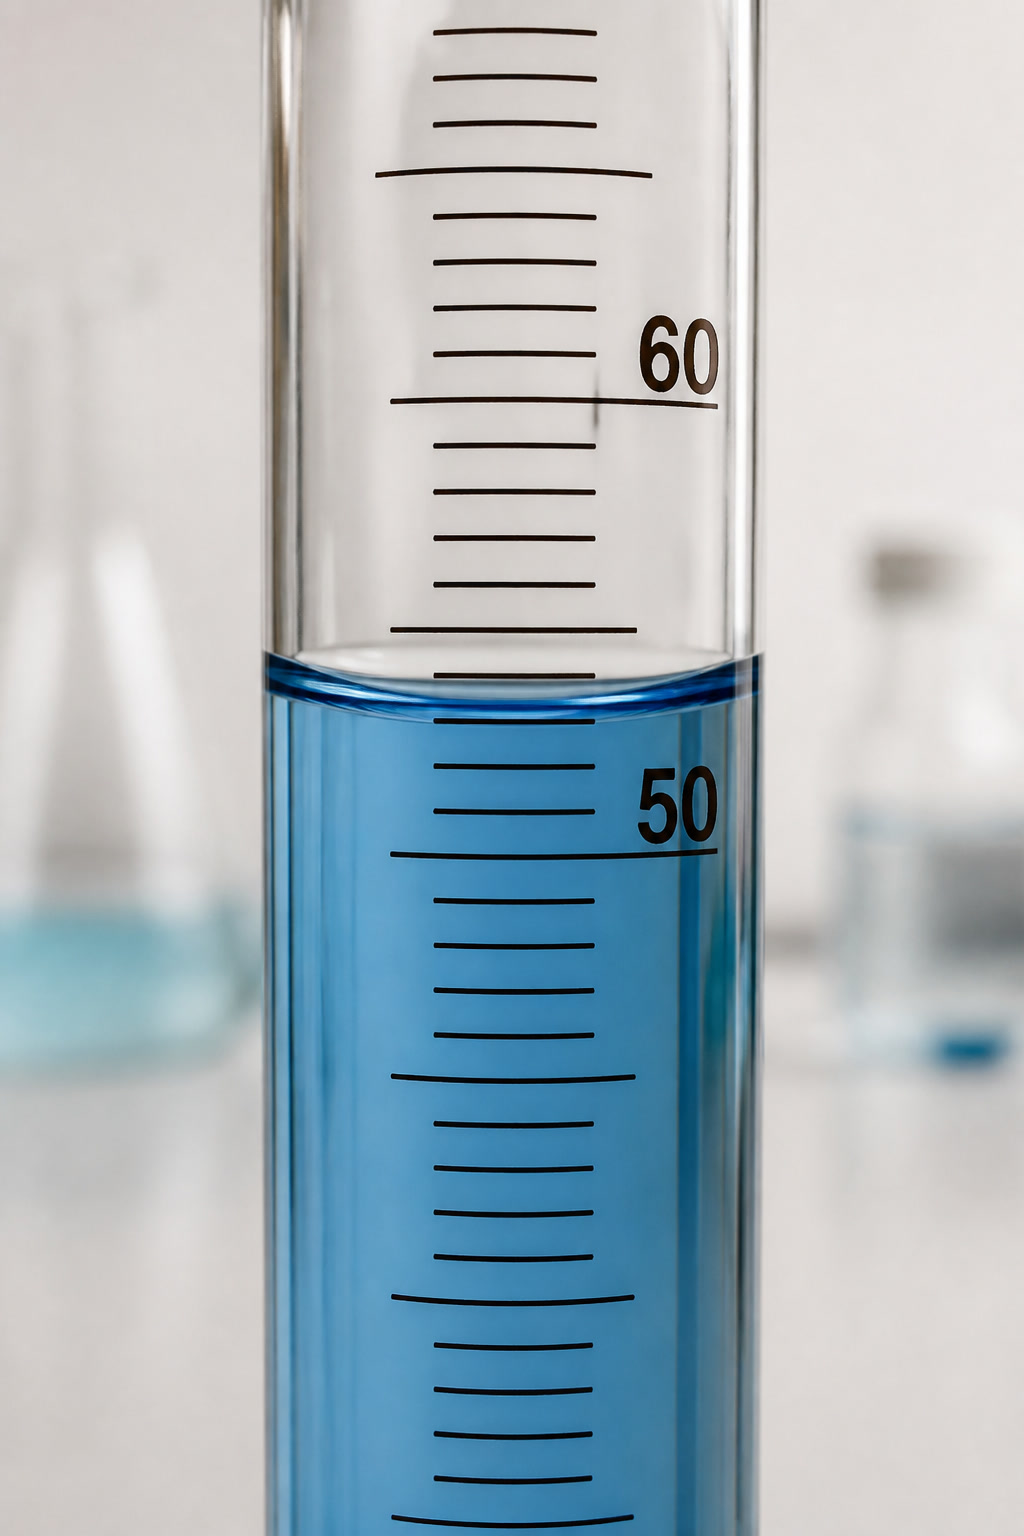
\includegraphics[width=0.3\linewidth]{images/book1/ai/g6-volume-cylinder.jpg}

{\small The \omterm{met:g6:mass-and-volume:cylinder}{meniscus} up close: read the flat middle of the curve, with your eye at its level.}
\end{omfigure}

\section{Measuring solids --- even lumpy ones}

A brick-shaped \omterm{def:g3:solids-liquids-gases:solid}{solid} surrenders to the ruler: length times width
times height gives its \omterm{def:g6:mass-and-volume:volume}{volume} in \unit{cm^3}, as your mathematics
course showed. But what of a pebble, a key, a plum? No ruler fits
a lump. The answer is two thousand years old, and it came out of a
bathtub.

\begin{proposition}[Displacement]\label{prop:g6:mass-and-volume:displacement}
A \omterm{def:g3:solids-liquids-gases:solid}{solid} lowered completely underwater pushes aside --- displaces
--- exactly its own \omterm{def:g6:mass-and-volume:volume}{volume} of water. The water level's rise
\omterm{def:g6:measurement-in-science:measuring}{measures} the intruder: lumpy or smooth, the water molds itself to
every dent and bump.
\end{proposition}

\begin{method}[Volume by the rise of water]\label{met:g6:mass-and-volume:rise}
\begin{enumerate}
  \item pour water into a measuring cylinder --- enough to cover
        the object --- and read the \omterm{def:g6:mass-and-volume:volume}{volume}: say \qty{120}{mL};
  \item tie a thread to the object and lower it gently until fully
        underwater, no splash, no touching the walls;
  \item read again: say \qty{145}{mL};
  \item subtract: $145 - 120 = 25$ --- the object's \omterm{def:g6:mass-and-volume:volume}{volume} is
        \qty{25}{cm^3} (millilitres of rise, centimetre-cubes of
        stone: the same thing).
\end{enumerate}
\end{method}

\begin{omfigure}
\begin{tikzpicture}[scale=0.85]
  \draw[thick] (0.8,0) -- (0.8,3.6) (2.6,0) -- (2.6,3.6)
    (0.8,0) -- (2.6,0);
  \fill[omDef, opacity=0.2] (0.8,0.05) rectangle (2.6,2.0);
  \draw[omDef, very thick] (0.8,2.0) -- (2.6,2.0);
  \node[right, font=\footnotesize] at (2.7,2.0) {120};
  \node[below, font=\small] at (1.7,-0.3) {before};
  \draw[thick] (6.2,0) -- (6.2,3.6) (8.0,0) -- (8.0,3.6)
    (6.2,0) -- (8.0,0);
  \fill[omDef, opacity=0.2] (6.2,0.05) rectangle (8.0,2.42);
  \draw[omDef, very thick] (6.2,2.42) -- (8.0,2.42);
  \node[right, font=\footnotesize] at (8.1,2.42) {145};
  \draw (7.1,3.6) -- (7.1,1.0);
  \fill[omExo] (7.1,0.75) ellipse (0.4 and 0.3);
  \node[below, font=\small] at (7.1,-0.3)
    {after: the pebble, fully under};
  \draw[-Stealth, omThm, thick] (4.0,2.0) -- (5.6,2.35);
  \node[below, font=\small, omThm] at (4.8,1.9)
    {rise: \qty{25}{mL}};
\end{tikzpicture}

{\small The rise method: the water climbs by exactly the pebble's
\omterm{def:g6:mass-and-volume:volume}{volume} --- $145 - 120 = \qty{25}{cm^3}$ of pebble.}
\end{omfigure}

\begin{example}[The crown in the bathtub]\label{ex:g6:mass-and-volume:archimedes}
The old story: a king suspected his goldsmith had thinned the royal
crown's gold with silver, and asked the scientist Archimedes to
find out without harming the crown. Stepping into a full bath,
Archimedes watched the water slosh over the rim --- and saw in a
flash that the overflow measured his own body's \omterm{def:g6:mass-and-volume:volume}{volume}, lumps and
all. Legend says he ran through the streets shouting ``Eureka!''
--- \emph{I have found it!} How the crown's \omterm{def:g6:mass-and-volume:volume}{volume} unmasked the
fraud needs one more idea, two chapters ahead; the bathtub gave him
the \omterm{def:g6:mass-and-volume:volume}{volume} of \emph{anything}.
\end{example}

\section{Mass and volume are different answers}

\begin{example}[Same volume, different mass]\label{ex:g6:mass-and-volume:different}
Fill two identical \qty{25}{cL} glasses, one with water, one with
honey, and weigh them (subtracting the glasses): the honey glass
holds noticeably more \omterm{def:g3:measuring-mass:units}{grams} in the very same room. Same \omterm{def:g6:mass-and-volume:volume}{volume},
different \omterm{def:g3:measuring-mass:mass}{mass}. And a \omterm{def:g6:mass-and-volume:volume}{litre} of \omterm{def:g2:air-around-us:air}{air} weighs hardly more than a \omterm{def:g3:measuring-mass:units}{gram},
in the room where a \omterm{def:g6:mass-and-volume:volume}{litre} of water weighs a full \omterm{def:g3:measuring-mass:units}{kilogram}. Room
and stuff are truly different bookkeepers --- hold that thought
firmly: it becomes a law, with a name, in the last chapter of this
year.
\end{example}

\begin{remark}[Weighing what cannot stand alone]\label{rem:g6:mass-and-volume:tare}
How to weigh flour without weighing its bowl? Modern balances have
a button for it: set the empty bowl on the pan, press --- the
display resets to zero --- then pour: the balance now reports the
flour alone. The maneuver is called \emph{taring}. Without the
button, weigh twice and subtract: bowl-with-flour minus empty
bowl. Either way, it is the fair-start rule again: begin from an
honest zero.
\end{remark}

\section{Exercises}

\begin{exercise}[$\star$]\label{exo:g6:mass-and-volume:1}
What question does \omterm{def:g6:mass-and-volume:volume}{volume} answer, and what question does \omterm{def:g3:measuring-mass:mass}{mass}
answer? Give the two chief \omterm{def:g6:measurement-in-science:measuring}{units} of each.
\end{exercise}

\begin{exercise}[$\star$]\label{exo:g6:mass-and-volume:2}
Convert: \qty{2}{L} to \unit{cm^3}; \ \qty{350}{mL} to
\unit{cm^3}; \ \qty{1500}{cm^3} to \omterm{def:g6:mass-and-volume:volume}{litres}; \ half a \omterm{def:g6:mass-and-volume:volume}{litre} to
millilitres.
\end{exercise}

\begin{exercise}[$\star$]\label{exo:g6:mass-and-volume:3}
Why must a measuring cylinder be read at eye level, on the table,
at the bottom of the \omterm{met:g6:mass-and-volume:cylinder}{meniscus}? Name the mistake each rule
prevents.
\end{exercise}

\begin{exercise}[$\star$]\label{exo:g6:mass-and-volume:4}
A cylinder reads \qty{200}{mL}; with a plum lowered in, it reads
\qty{265}{mL}. What is the plum's \omterm{def:g6:mass-and-volume:volume}{volume}, in \unit{cm^3}?
\end{exercise}

\begin{exercise}[$\star$]\label{exo:g6:mass-and-volume:5}
Why does the rise method work even for a lumpy pebble, when no
ruler could \omterm{def:g6:measurement-in-science:measuring}{measure} it? Which proposition answers?
\end{exercise}

\begin{exercise}[$\star$]\label{exo:g6:mass-and-volume:6}
A brick-shaped eraser \omterm{def:g6:measurement-in-science:measuring}{measures} \qty{5}{cm} by \qty{2}{cm} by
\qty{1}{cm}. Its \omterm{def:g6:mass-and-volume:volume}{volume}? Check-plan: how would you confirm it
with the rise method?
\end{exercise}

\begin{exercise}[$\star$]\label{exo:g6:mass-and-volume:7}
To weigh rice: empty bowl \qty{280}{g}; bowl with rice
\qty{745}{g}. How much rice? What button does the same job in one
step?
\end{exercise}

\begin{exercise}[$\star$]\label{exo:g6:mass-and-volume:8}
Which has the greater \omterm{def:g6:mass-and-volume:volume}{volume}, a \omterm{def:g3:measuring-mass:units}{kilogram} of feathers or a \omterm{def:g3:measuring-mass:units}{kilogram}
of iron? Which has the greater \omterm{def:g3:measuring-mass:mass}{mass}? (Answer both carefully.)
\end{exercise}

\begin{exercise}[$\star\star$]\label{exo:g6:mass-and-volume:9}
The rise method fails for a cork: it \omterm{def:g1:floating-and-sinking:words}{floats}. Propose a fix that
still uses the cylinder --- and say what must be subtracted if
your fix uses a helper object.
\end{exercise}

\begin{exercise}[$\star\star$]\label{exo:g6:mass-and-volume:10}
A juice carton claims \qty{1}{L}. Poured out, it fills a
\qty{250}{mL} glass three times, and the fourth glass only up to
the \qty{200}{mL} mark. Was the claim honest? By how much?
\end{exercise}

\begin{exercise}[$\star\star$]\label{exo:g6:mass-and-volume:11}
A necklace is lowered into a cylinder reading \qty{80.0}{mL}; it
rises to \qty{83.5}{mL}. The jeweler claims the necklace contains
\qty{5}{cm^3} of gold. Could the claim be true? What, exactly,
did the water \omterm{def:g6:measurement-in-science:measuring}{measure}?
\end{exercise}

\begin{exercise}[$\star\star\star$]\label{exo:g6:mass-and-volume:12}
Design a bathtub-style check of
\cref{prop:g6:mass-and-volume:displacement} itself, using a
brick-shaped object whose \omterm{def:g6:mass-and-volume:volume}{volume} the ruler already knows. Describe
the steps, predict the two cylinder readings for a
$4 \times 3 \times 2$ \omterm{def:g2:measuring-length:units}{centimetre} block lowered into
\qty{150}{mL}, and state what result would prove the proposition
wrong.
\end{exercise}

\section{Problem: Bottling Day at the Orchard}

\begin{problem}[{Weekend problem --- pressing day at the orchard;
litres into bottles, crates onto scales; the pebble in the
jug}]\label{pb:g6:mass-and-volume:1}
The orchard presses its apples today, and every helper gets a
measuring job.

\medskip\noindent\textbf{Part I --- Juice by the \omterm{def:g6:mass-and-volume:volume}{litre}.}
The press has filled a \qty{20}{L} barrel.
\begin{enumerate}
  \item How many \omterm{def:g6:mass-and-volume:volume}{cubic centimetres} is \qty{20}{L}?
  \item The juice is bottled in \qty{75}{cL} bottles. How many
        \emph{full} bottles does the barrel give?
  \item How much juice is left over after the last full bottle, in
        centilitres?
  \item The leftover is poured into glasses of \qty{25}{cL}. How
        many glasses does it fill?
\end{enumerate}

\medskip\noindent\textbf{Part II --- Crates on the scale.}
\begin{enumerate}[resume]
  \item An empty bottle has \omterm{def:g3:measuring-mass:mass}{mass} \qty{450}{g}. Using Part I, what
        is the \omterm{def:g3:measuring-mass:mass}{mass} of the juice in one full bottle, if a \omterm{def:g6:mass-and-volume:volume}{litre} of
        juice has a \omterm{def:g3:measuring-mass:mass}{mass} of about \qty{1}{kg}? (Work in \omterm{def:g3:measuring-mass:units}{grams}.)
  \item So what does one full bottle weigh altogether?
  \item A wooden crate weighs \qty{2}{kg} empty and carries six
        full bottles. Total \omterm{def:g3:measuring-mass:mass}{mass} of a loaded crate?
  \item The van may carry \qty{200}{kg} of crates. How many loaded
        crates may it take? (Whole crates only.)
\end{enumerate}

\medskip\noindent\textbf{Part III --- The pebble in the jug.}
Little Tom drops a pebble into a full \qty{1}{L} jug of juice, and
juice overflows onto the table.
\begin{enumerate}[resume]
  \item The mopped-up overflow \omterm{def:g6:measurement-in-science:measuring}{measures} \qty{40}{mL}. What did the
        spill \omterm{def:g6:measurement-in-science:measuring}{measure} about the pebble, and by which proposition?
  \item After the pebble is fished out, how much juice remains in
        the jug?
  \item Tom protests: ``The pebble is small --- look, it hides in
        my fist!'' His sister answers with a measuring cylinder:
        she puts the pebble in \qty{100}{mL} of water. What
        reading proves the spill told the truth?
  \item Bonus bookkeeping: the pebble weighs \qty{104}{g} on the
        kitchen scale. Without any new idea, can you yet say
        whether pebble-stuff is heavier or lighter than
        juice-stuff \emph{for the same room taken}? Compare
        \qty{104}{g} of pebble in \qty{40}{cm^3} with what \omterm{def:g3:measuring-mass:mass}{mass} of
        juice would fill those same \qty{40}{cm^3} --- and keep
        your conclusion warm for the density chapter.
\end{enumerate}
\end{problem}
